\documentclass[a4paper,12pt]{report}

\usepackage{cmap}
\usepackage[T2A]{fontenc}
\usepackage[utf8]{inputenc}
\usepackage[english,russian]{babel}
\usepackage{listings}
\usepackage{amsmath}
\usepackage{float}
\usepackage{csquotes}
\usepackage{mathtools}
\usepackage{hyphenat}
\usepackage{amsfonts}
\usepackage{upgreek}

\usepackage{xcolor}
\usepackage{hyperref}

\usepackage{graphicx}
\graphicspath{ {./images/} }

\definecolor{dkgreen}{rgb}{0,0.6,0}
\definecolor{gray}{rgb}{0.5,0.5,0.5}
\definecolor{mauve}{rgb}{0.58,0,0.82}

\lstset{
    language=Python,                 % выбор языка для подсветки (здесь это С)
    basicstyle=\small\sffamily, % размер и начертание шрифта для подсветки кода
    numbers=left,               % где поставить нумерацию строк (слева\справа)
    numberstyle=\tiny,           % размер шрифта для номеров строк
    stepnumber=1,                   % размер шага между двумя номерами строк
    numbersep=5pt,                % как далеко отстоят номера строк от подсвечиваемого кода
    aboveskip=3mm,
    belowskip=3mm,
    showstringspaces=false,
    columns=flexible,
    captionpos=b, 
    basicstyle={\small\ttfamily},
    numbers=left,
    numberstyle=\tiny\color{gray},
    keywordstyle=\color{blue},
    commentstyle=\color{mauve},
    stringstyle=\color{dkgreen},
    breaklines=true,
    breakatwhitespace=true,
    tabsize=3
}

\title{Лабораторная работа №8\\Фильтрация и свёртка}
\author{Кобыжев Александр}
\date{\today}

\begin{document}

\maketitle
\tableofcontents
\listoffigures
\lstlistoflistings

\maketitle

\chapter{Упражнение 8.1}

В данном упражнении нас просят открыть \texttt{chap08.ipynb}, прочитать пояснения, а также запустить примеры. 

Если увеличивать ширину гауссова окна STD без увеличения количества элементов в окне M, это окно становится ближе к прямоугольному, более высокие частоты подавляются хуже, и следующие параметры проявляются боковым лепестком.

\chapter{Упражнение 8.2}

Начнём с гауссовского аналога:

\begin{lstlisting}[caption=Визуализация гауссовского сигнала]
gaussian = scipy.signal.gaussian(M=64, std=2)
gaussian /= sum(gaussian)
thinkplot.plot(gaussian)
thinkplot.config(xlabel='Index')
\end{lstlisting}

\begin{figure}[H]
        \centering
        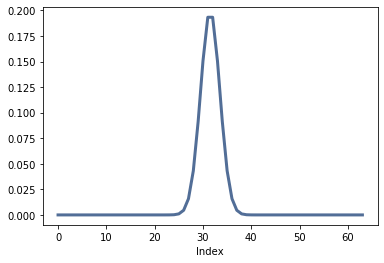
\includegraphics[width=0.75\textwidth]{lab8_fig2_1.png}
        \caption{Визуализация гауссовского сигнала}
        \label{fig:lab8_fig2_1}
\end{figure}

Вот как выглядит БПФ:

\begin{lstlisting}[caption=Визуализация БПФ]
fft_gaussian = np.fft.fft(gaussian)
thinkplot.plot(abs(fft_gaussian))
thinkplot.config(xlabel='Frequency (Hz)', ylabel='Amplitude')
\end{lstlisting}

\begin{figure}[H]
        \centering
        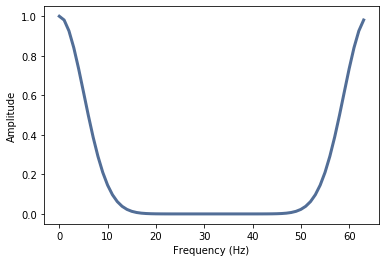
\includegraphics[width=0.75\textwidth]{lab8_fig2_2.png}
        \caption{Визуализация БПФ}
        \label{fig:lab8_fig2_2}
\end{figure}

Если мы повернём отрицательные частоты влево, то сможем яснее увидеть, что это гауссово, по крайней мере приблизительно.

\begin{lstlisting}[caption=Визуализация гауссовского сигнала]
N = len(gaussian)
fft_rolled = np.roll(fft_gaussian, N//2)
thinkplot.plot(abs(fft_rolled))
thinkplot.config(xlabel='Frequency (Hz)', ylabel='Amplitude')
\end{lstlisting}

\begin{figure}[H]
        \centering
        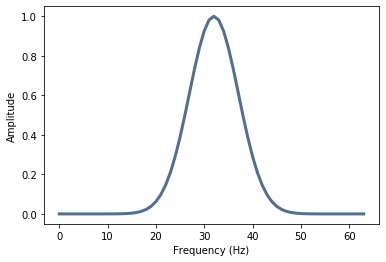
\includegraphics[width=0.75\textwidth]{lab8_fig2_3.png}
        \caption{Визуализация гауссовского сигнала}
        \label{fig:lab8_fig2_3}
\end{figure}

Эта функция отображает окно Гаусса и его БПФ друг с другом.

\begin{lstlisting}[caption=Функция \texttt{plot\_gaussian}]
def plot_gaussian(std):
    M = 64
    gaussian = scipy.signal.gaussian(M=M, std=std)
    gaussian /= sum(gaussian)
    
    thinkplot.preplot(num=2, cols=2)
    thinkplot.plot(gaussian)
    thinkplot.config(xlabel='Time', legend=False)

    fft_gaussian = np.fft.fft(gaussian)
    fft_rolled = np.roll(fft_gaussian, M//2)
    
    thinkplot.subplot(2)
    thinkplot.plot(abs(fft_rolled))
    thinkplot.config(xlabel='Frequency')

    
plot_gaussian(2)
\end{lstlisting}

\begin{figure}[H]
        \centering
        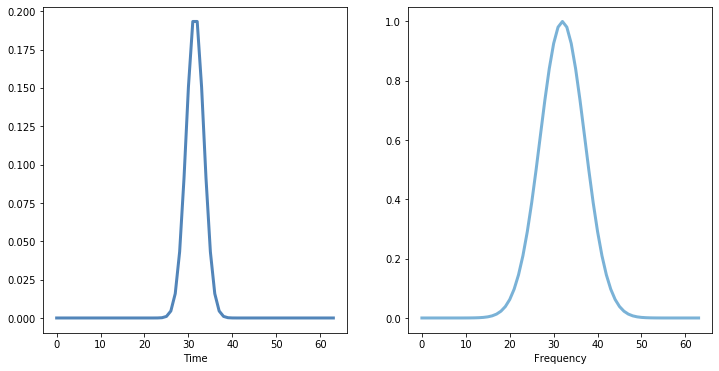
\includegraphics[width=0.75\textwidth]{lab8_fig2_4.png}
        \caption{Визуализация окна Гаусса и его БПФ}
        \label{fig:lab8_fig2_4}
\end{figure}

Теперь мы можем сделать взаимодействие, которое показывает, что происходит при изменении \texttt{std}.

\begin{lstlisting}[caption=Изменение \texttt{std}]
from ipywidgets import interact, interactive, fixed
import ipywidgets as widgets

slider = widgets.FloatSlider(min=0.1, max=10, value=2)
interact(plot_gaussian, std=slider);
\end{lstlisting}

\begin{figure}[H]
        \centering
        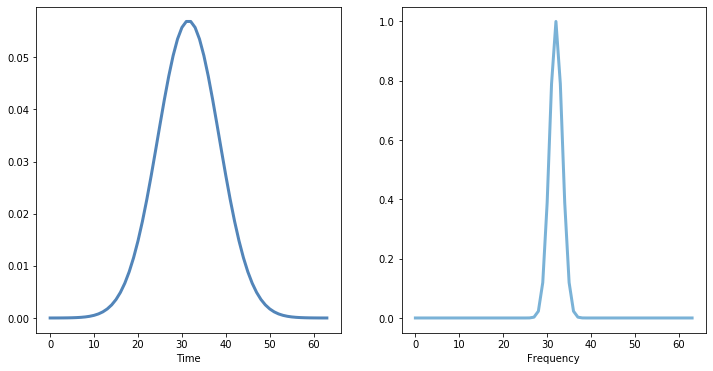
\includegraphics[width=0.75\textwidth]{lab8_fig2_5.png}
        \caption{Изменение \texttt{std}}
        \label{fig:lab8_fig2_5}
\end{figure}

По мере увеличения \texttt{std} Гауссовский становится шире, а его БПФ сужается.

С точки зрения непрерывной математики, если

$f(x) = e^{-a x^2}$

который является гауссовским со средним 0 и стандартным отклонением $1/a$, его преобразование Фурье имеет вид

$F(k) = \sqrt{\frac{\pi}{a}} e^{-\pi^2 k^2/a}$

который является гауссовским со стандартным отклонением $a / \pi^2$. Таким образом, существует обратная зависимость между стандартными отклонениями $f$ и $F$.

\chapter{Упражнение 8.3}

Создадим 1-секундную волну с частотой дискретизации 44 кГц.

\begin{lstlisting}[caption=Создание сигнала]
signal = thinkdsp.SquareSignal(freq=440)
wave = signal.make_wave(duration=1.0, framerate=44000)
\end{lstlisting}

Затем создадим несколько окон. Выберем стандартное отклонение окна Гаусса, чтобы сделать его похожим на другие.

\begin{lstlisting}[caption=Создание различных окон]
M = 17
std = 2.5

gaussian = scipy.signal.gaussian(M=M, std=std)   
bartlett = np.bartlett(M)
blackman = np.blackman(M)
hamming = np.hamming(M)
hanning = np.hanning(M)

windows = [gaussian, blackman, hamming, hanning]
names = ['gaussian', 'blackman', 'hamming', 'hanning']

for window in windows:
    window /= sum(window)
\end{lstlisting}

Теперь посмотрим, как выглядят эти окна.

\begin{lstlisting}[caption=Визуализация окон]
thinkplot.preplot(4)
for window, name in zip(windows, names):
    thinkplot.plot(window, label=name)

thinkplot.config(xlabel='Index', legend=True, loc='center bottom')
\end{lstlisting}

\begin{figure}[H]
        \centering
        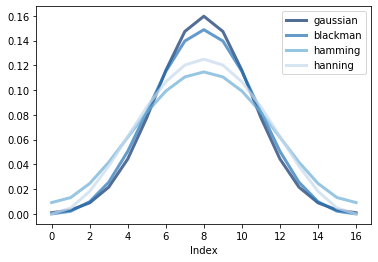
\includegraphics[width=0.75\textwidth]{lab8_fig3_1.png}
        \caption{Визуализация окон}
        \label{fig:lab8_fig3_1}
\end{figure}

Они выглядят довольно похоже, но по Гауссу и Блэкману немного выше. Посмотрим, как выглядят их ДПФ:

\begin{lstlisting}[caption=Функция \texttt{plot\_window\_dfts}]
def plot_window_dfts(windows, names):
    thinkplot.preplot(5)

    for window, name in zip(windows, names):
        padded = thinkdsp.zero_pad(window, len(wave))
        dft_window = np.fft.rfft(padded)
        thinkplot.plot(abs(dft_window), label=name)
\end{lstlisting}

\begin{lstlisting}[caption=Визуализация ДПФ]
plot_window_dfts(windows, names)
thinkplot.config(xlabel='Frequency (Hz)', loc='upper right')
\end{lstlisting}

\begin{figure}[H]
        \centering
        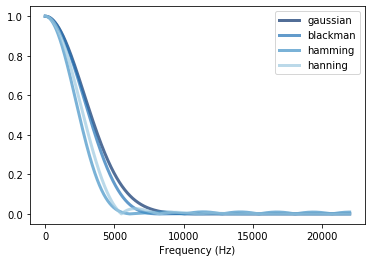
\includegraphics[width=0.75\textwidth]{lab8_fig3_2.png}
        \caption{Визуализация ДПФ}
        \label{fig:lab8_fig3_2}
\end{figure}

Тоже очень похоже, но похоже, что Гауссово падает быстрее всех, Блэкман - самым медленным, а у Ханнинга самые заметные боковые лепестки.

\begin{lstlisting}[caption=Визуализация ДПФ]
plot_window_dfts(windows, names)
thinkplot.config(xlabel='Frequency (Hz)', yscale='log', 
                 loc='lower left')
\end{lstlisting}

\begin{figure}[H]
        \centering
        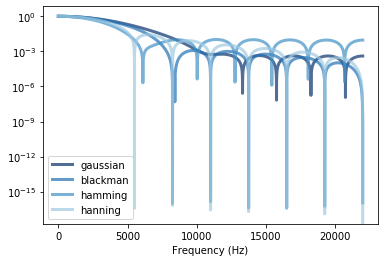
\includegraphics[width=0.75\textwidth]{lab8_fig3_3.png}
        \caption{Визуализация ДПФ}
        \label{fig:lab8_fig3_3}
\end{figure}

В логарифмической шкале мы видим, что сначала значения Хэмминга и Хеннинга падают быстрее, чем два других. И окна Хэмминга и Гаусса, кажется, имеют самые стойкие боковые лепестки. Окно Ханнинга, кажется, имеет наилучшее сочетание быстрого спада и минимальных боковых лепестков.

\chapter{Выводы}

Во время выполнения лабораторной работы получены навыки работы с концепцией свёртки и теоремой свёртки, а также научился применять эти знания на практике.

\end{document}